\documentclass{standalone}
\usepackage{tikz}
\begin{document}

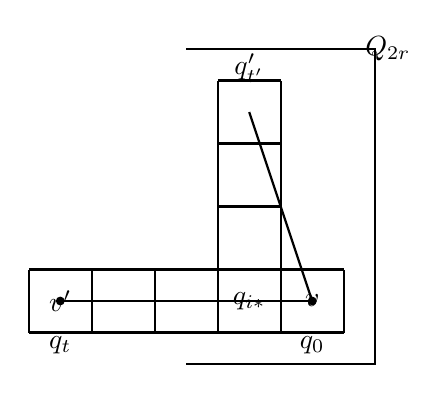
\begin{tikzpicture}[scale=0.8]
    % Draw grid
    \draw[step=1cm,black,thick] (0,0) grid (5,1);
    \draw[step=1cm,black,thick] (3,1) grid (4,4);

    % Labels
    \node at (0.5,0.5) {$v'$};
    \node at (4.5,0.5) {$v$};
    \node at (0.5,-0.2) {$q_t$};
    \node at (4.5,-0.2) {$q_0$};
    \node at (3.5,4.2) {$q'_{t'}$};
    \node at (3.5,0.5) {$q_{i*}$};

    % Path lines
    \draw[thick] (0.5,0.5) -- (4.5,0.5);
    \draw[thick] (4.5,0.5) -- (3.5,3.5);

    % Point markers
    \fill (0.5,0.5) circle (2pt);
    \fill (4.5,0.5) circle (2pt);

    % Outer box
    \draw[thick] (2.5,4.5) -- (5.5,4.5) -- (5.5,-0.5) -- (2.5,-0.5);

    % Q2r label
    \node at (5.7,4.5) {$Q_{2r}$};

\end{tikzpicture}

\end{document}